\documentclass[11pt,a4paper]{article}
% Paquetes esenciales y codificación
\usepackage[utf8]{inputenc}
\usepackage[T1]{fontenc}
\usepackage[spanish]{babel}
\usepackage[margin=2.5cm]{geometry}
\usepackage{hyperref}
\usepackage{graphicx}
\usepackage{float}
\usepackage{xcolor}
\usepackage{booktabs}
\usepackage{listings}
% Configuración de hipervínculos y código
\hypersetup{colorlinks=true, linkcolor=blue, urlcolor=cyan}
\definecolor{codegray}{rgb}{0.95,0.95,0.95}
\definecolor{codeblue}{rgb}{0.1,0.2,0.8}
\lstset{
backgroundcolor=\color{codegray},
basicstyle=\ttfamily\footnotesize,
keywordstyle=\color{codeblue}\bfseries,
frame=single,
breaklines=true
}
\title{\textbf{Documento de Arquitectura y Especificación de Requisitos} \\ Sistema de Control de Acceso}
\author{Ingeniería de Sistemas Integrados}
\date{Octubre 2026}
\begin{document}
\maketitle
\tableofcontents
\newpage
% ==========================================
% SECCIÓN 1: INTRODUCCIÓN Y TOPOLOGÍA GENERAL
% ==========================================
\section{Introducción y Topología General}
El presente documento detalla la arquitectura, la especificación de requisitos y el diseño de un Sistema de Control de Acceso Físico Inteligente. Este sistema ha sido construido sobre hardware de grado embebido (SoC BCM2711 en una Raspberry Pi 4) operando bajo un sistema operativo Linux minimalista compilado a la medida mediante \textbf{Yocto Project} (rama \textit{Scarthgap/Wrynose}).
El presente documento detalla la arquitectura, la especificación de requisitos y el diseño de un Sistema de Control de Acceso Físico Inteligente. Este sistema ha sido construido sobre hardware de grado embebido (SoC BCM2711 en una Raspberry Pi 4) operando bajo un sistema operativo Linux minimalista compilado a la medida mediante \textbf{Yocto Project} (rama \textit{Wrynose 6.0})
\subsection{Topología Conceptual}
La infraestructura se divide arquitectónicamente en tres dominios físicos y lógicos, diseñados para garantizar la degradación segura y la tolerancia a fallos:
\begin{enumerate}
\item \textbf{Capa de Hardware en el Borde:} Compuesta por la Raspberry Pi 4, la cual interactúa con el mundo físico mediante captura de video UVC y el cabezal GPIO. El hardware controla un relé de apertura (LED Verde), un indicador de estado de bloqueo (LED Rojo) y un lazo de seguridad para evacuación manual (Botón REX).

\item \textbf{Capa de Red Perimetral:} El sistema se acopla a la red corporativa mediante \texttt{systemd-networkd} (DHCP). Utiliza el protocolo asíncrono UDP para el transporte de paquetes RTP que contienen el video comprimido en el estándar H.264.

\item \textbf{Capa de Monitoreo Remoto:} Una estación de trabajo externa que recibe el flujo de video en vivo. Esta estación está totalmente desacoplada lógicamente de la toma de decisiones.
\end{enumerate}
\begin{figure}[H]
\centering

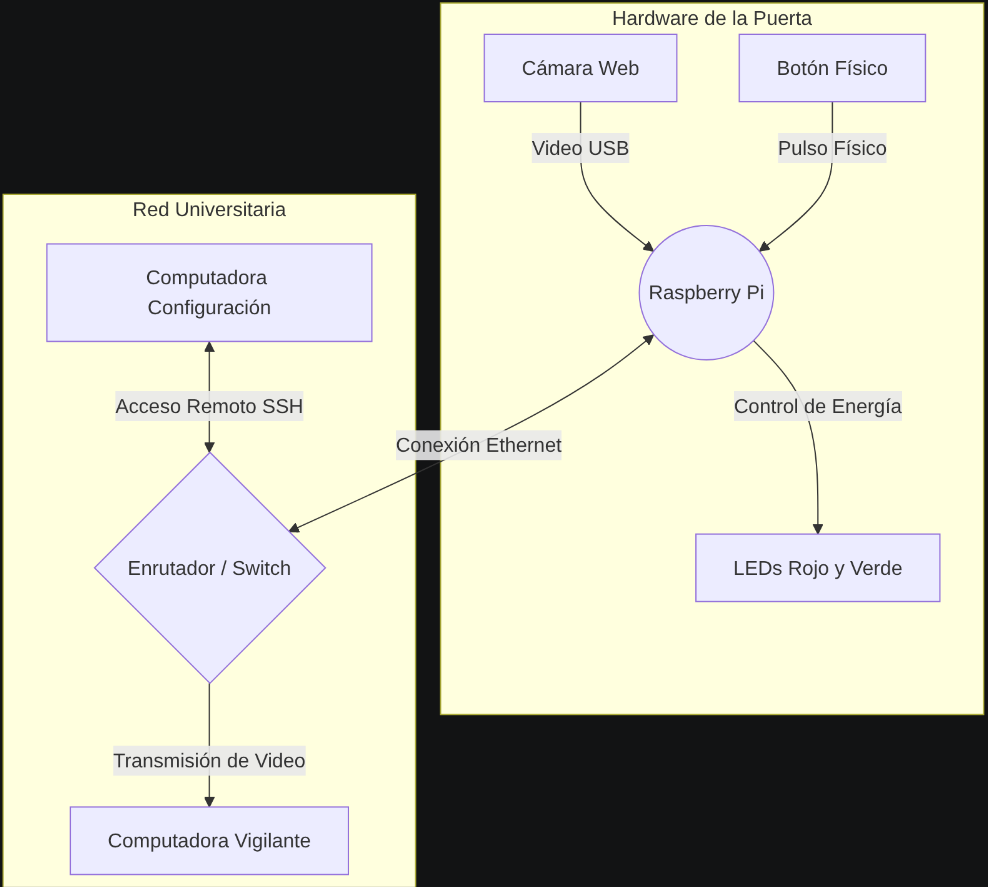
\includegraphics[width=0.70\textwidth]{Diagrama_general.png}
\caption{Diagrama General de Topología Física y Red}
\label{fig:topologia}
\end{figure}
\newpage
% ==========================================
% SECCIÓN 2: CASOS DE USO DEL SISTEMA
% ==========================================
\section{Análisis de Casos de Uso}
\subsection{Definición de Actores}
\begin{itemize}
\item \textbf{Ingeniero:} Personal técnico responsable del despliegue del firmware. Configura variables volátiles en el archivo de entorno.
\item \textbf{Vigilante:} Operador de la estación de seguridad central. Recibe de manera pasiva el video en tiempo real.
\item \textbf{Persona 1 (Autorizada):} Usuario legítimo que requiere ingresar o salir.
\item \textbf{Persona 2 (Intruso):} Entidad no autorizada que intenta vulnerar el perímetro ingresando furtivamente.
\end{itemize}
\begin{figure}[H]

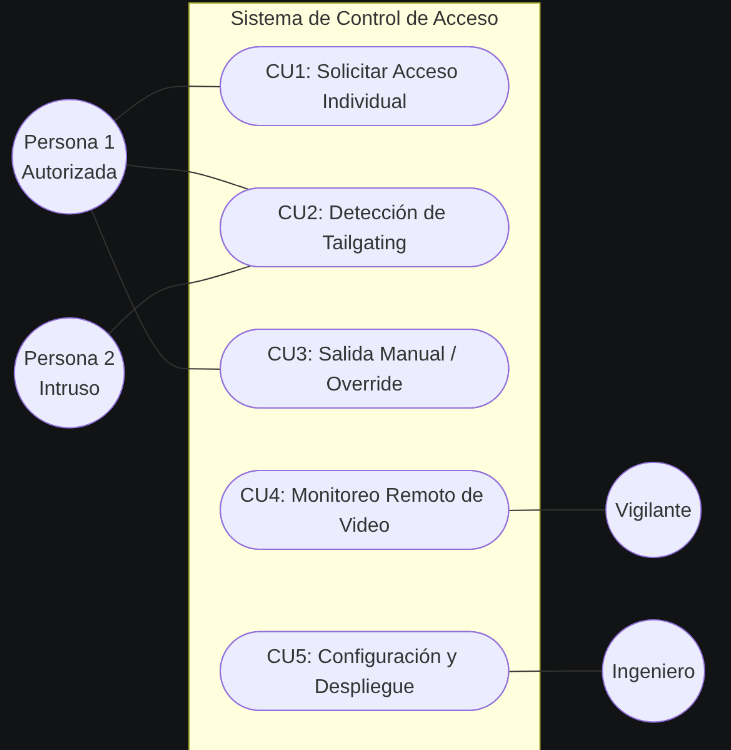
\includegraphics[width=0.8\textwidth]{Diagrama_de_casos.png}
\caption{Diagrama de Casos de Uso del Sistema}
\label{fig:casos_uso}
\end{figure}
\subsection{Especificación Detallada de Casos de Uso}
\begin{itemize}
\item \textbf{CU1 (Acceso Individual):} El sistema aísla un (1) solo rostro en el cuadro, autoriza el acceso activando el relevador por 3.0 segundos y asienta el evento en la bitácora.
\item \textbf{CU2 (Detección de Tailgating):} La IA devuelve un array con más de un rostro. Se bloquea la apertura, se dispara un evento para capturar evidencia fotográfica en el disco duro, y se levanta una alerta en el registro CSV.

 \item \textbf{CU3 (Salida Manual / Override):} La Persona 1 acciona el botón físico REX. El sistema detecta una interrupción de hardware (\texttt{FALLING\_EDGE}) en el GPIO, liberando la cerradura eléctrica por 3.0 segundos. \textit{Nota de Prototipo: Debido a limitaciones de componentes, se implementó con un pulsador Normalmente Abierto (NA), careciendo de seguridad Fail-Safe ante cortes de cableado.}
\item \textbf{CU4 (Monitoreo Remoto):} La Raspberry Pi codifica por hardware a H.264 y envía los paquetes UDP. Todo esto ocurre en un hilo separado de la IA.
\item \textbf{CU5 (Despliegue Zero-Touch):} \texttt{systemd} inicializa los servicios, espera 5 segundos a que la cámara USB se registre, e inicia la aplicación en modo autónomo (\texttt{Restart=always}).
\end{itemize}


% ==========================================
% SECCIÓN 3: ESPECIFICACIÓN Y TRAZABILIDAD
% ==========================================
\section{Especificación de Requisitos y Trazabilidad}
\subsection{Requisitos Funcionales (RF)}
\begin{table}[H]
\centering
\renewcommand{\arraystretch}{1.4}
\begin{tabular}{|c|p{8.5cm}|p{4.5cm}|}
\hline
\textbf{ID} & \textbf{Descripción del Requisito} & \textbf{Trazabilidad (Módulo)} \\
\hline
\textbf{RF-01} & \textbf{Acceso Individual:} La decisión de acceso debe correr fuera del hilo principal de GStreamer para evitar bloqueos. & \texttt{hilo\_ia.py} y \texttt{appsink pull-sample} \\
\hline
\textbf{RF-02} & \textbf{Tiempo de Decisión:} El sistema negará el acceso por omisión si pasan 10s sin detección. & \texttt{hilo\_ia.py} (\texttt{TIMEOUT}) \\
\hline
\textbf{RF-03} & \textbf{Prevención de Tailgating:} Detección de 2 o más rostros simultáneos denegará el acceso. & \texttt{hilo\_ia.py} (\texttt{len(cajas) > 1}) \\
\hline
\textbf{RF-04} & \textbf{Botón Override:} Existirá un botón de salida manual configurado con lógica tolerante a fallos y temporizador 3.0s. & \texttt{gpio\_ctrl.py} (\texttt{FALLING\_EDGE}) \\
\hline
\textbf{RF-05} & \textbf{Evidencia Forense:} Registros y capturas fotográficas ante violaciones deben persistir en almacenamiento físico. & \texttt{bitacora.py} y \texttt{Pad Probe} \\
\hline
\textbf{RF-06} & \textbf{Manejo de EOS:} Al detener el servicio se enviará señal EOS para asegurar la integridad de la última fotografía. & \texttt{main.py} (\texttt{\_apagado\_ordenado}) \\
\hline
\end{tabular}

\end{table}

% ==========================================
% SECCIÓN 4: DISEÑO DEL PIPELINE
% ==========================================
\section{Diseño Arquitectónico del Pipeline (GStreamer)}
El núcleo multimedia fue diseñado bajo el principio de asincronía estricta. Utilizando GStreamer, la topología extrae el video de la fuente y lo bifurca hacia tres consumidores independientes con capacidades y formatos diametralmente distintos.
\begin{figure}[H]
\centering
% Descomentar y cambiar el nombre de la imagen cuando la subas a tu plataforma
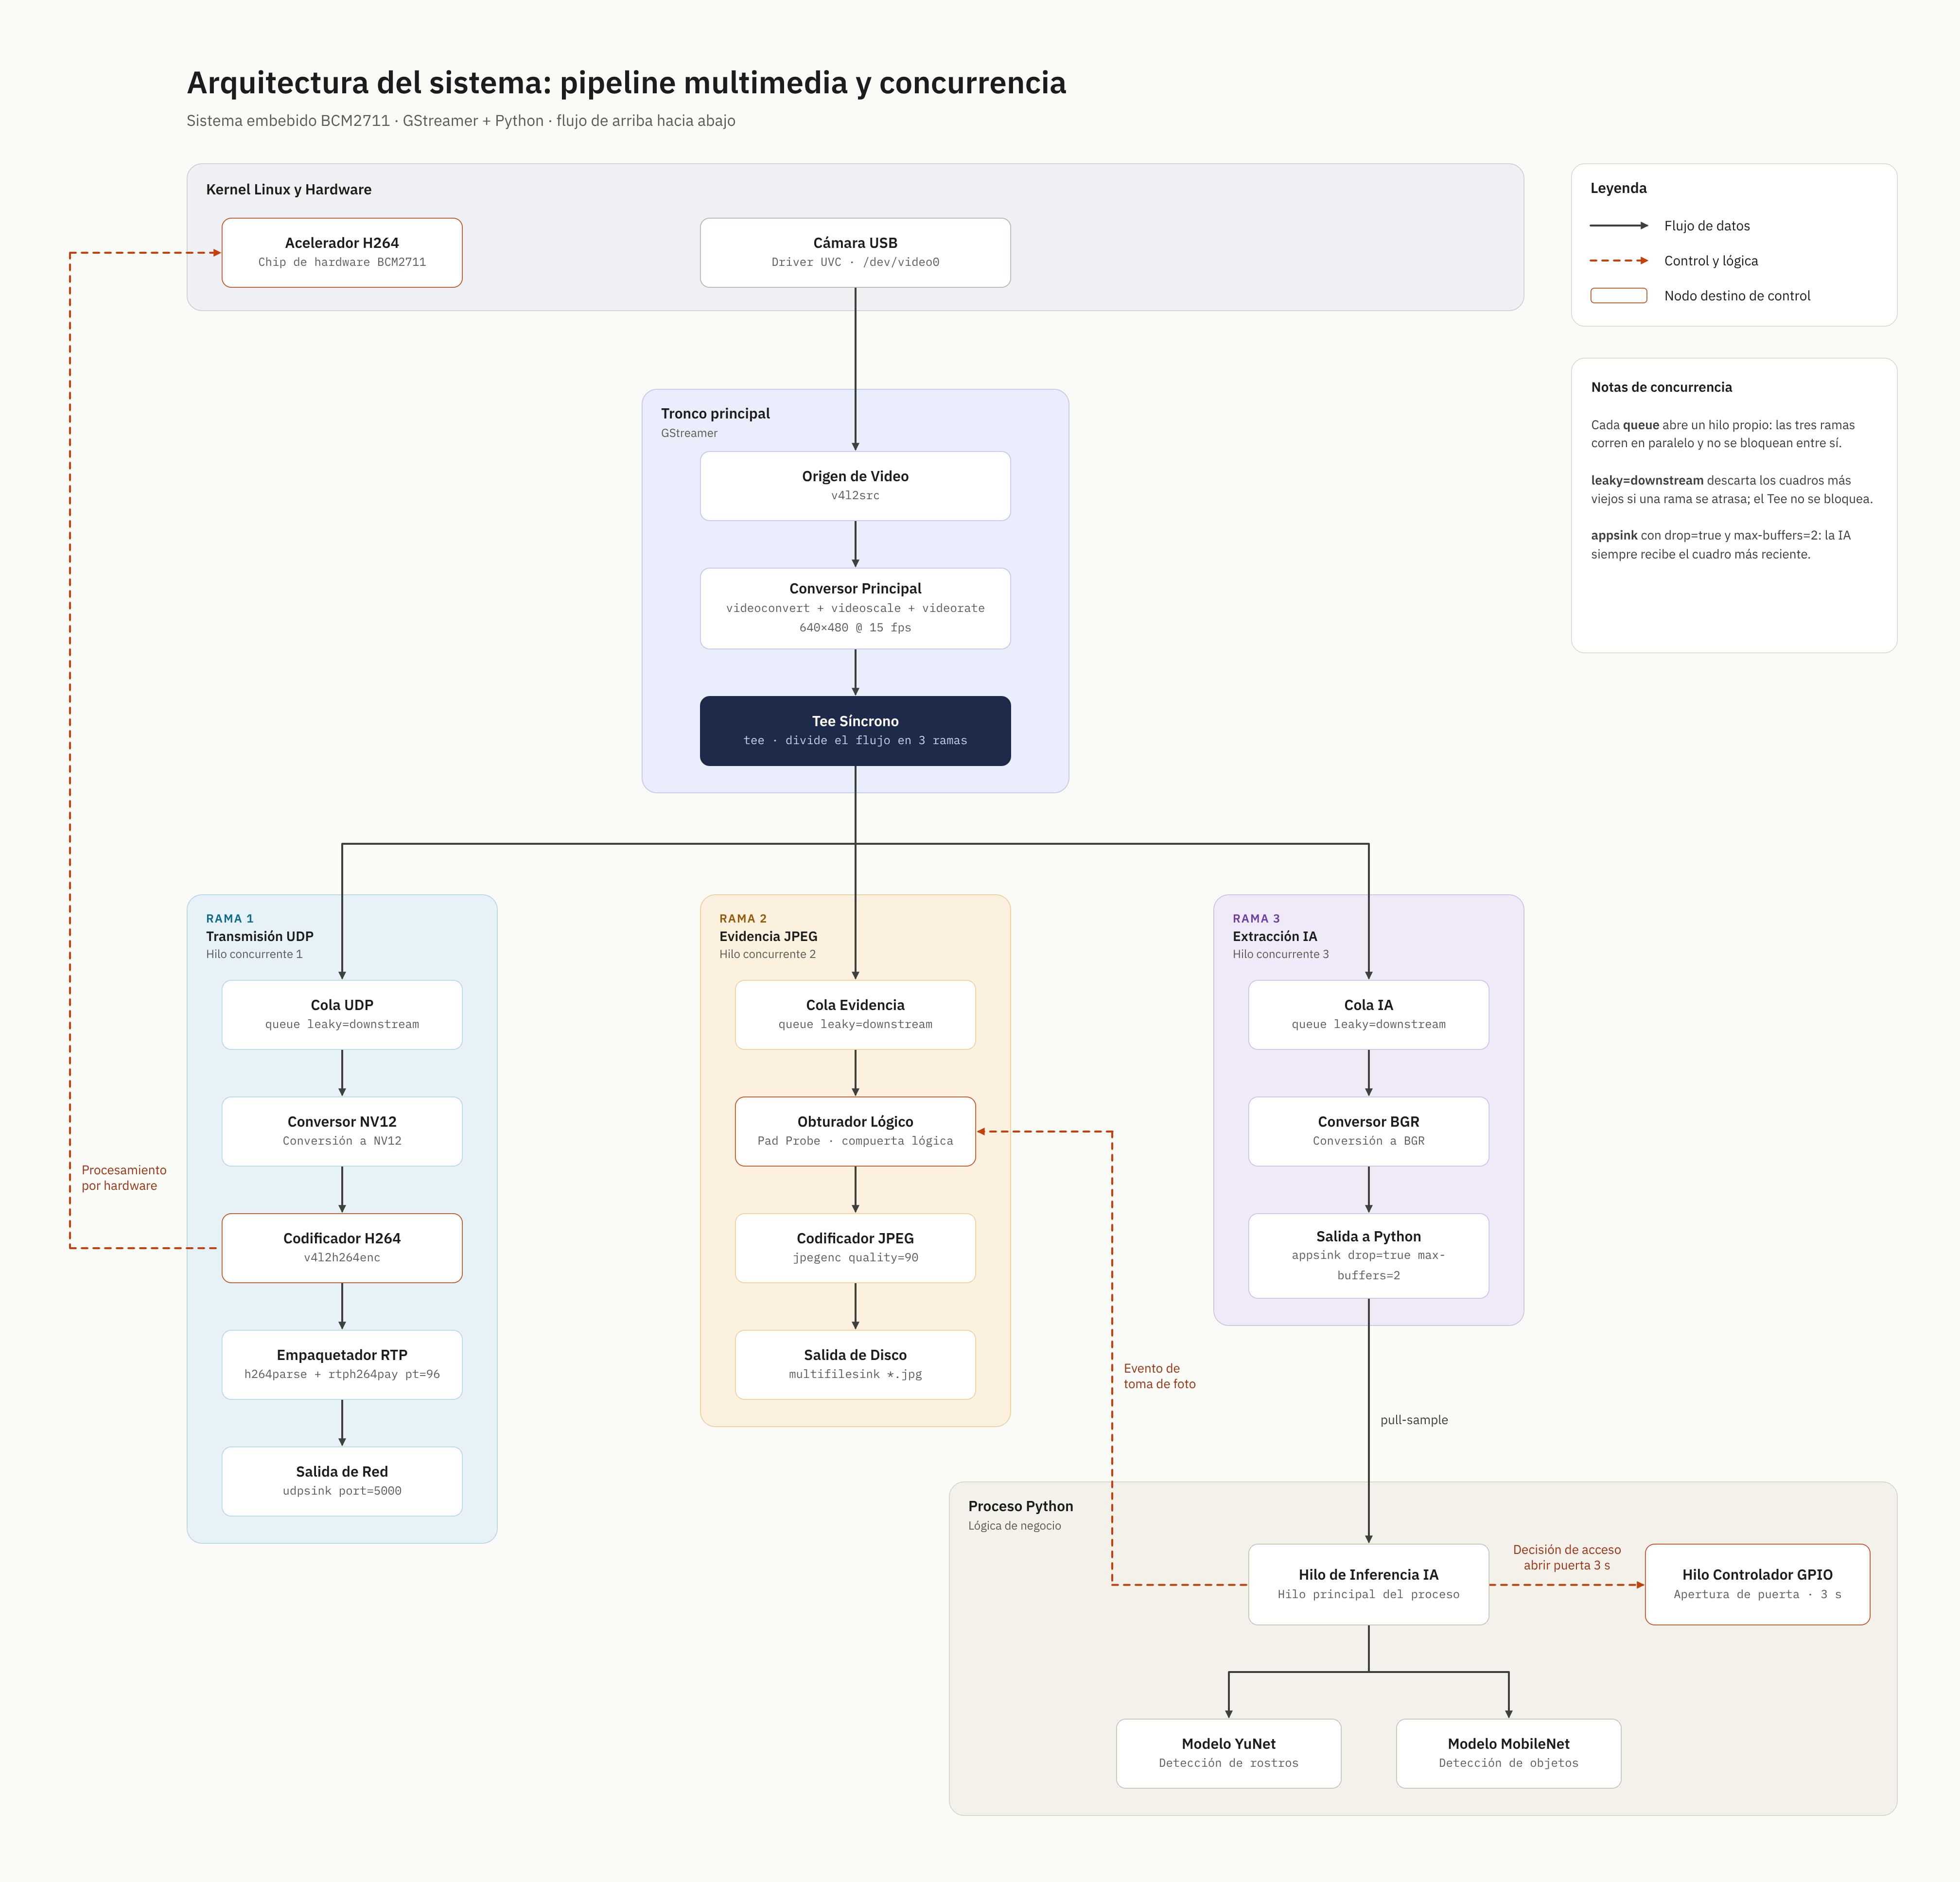
\includegraphics[width=\textwidth]{Pipeline.png}
\caption{Diagrama de Flujo Interno y Concurrencia del Pipeline Multimedia}
\label{fig:pipeline_detallado}
\end{figure}
\subsection{Justificación de Restricciones (Capsfilters)}
\begin{itemize}
\item \textbf{\texttt{video/x-raw, width=640, height=480, framerate=15/1}:} Se limitó la fuente original a resolución VGA a 15 fps. Procesar 1080p a 30fps mediante IA por CPU saturaría los núcleos ARM, induciendo temperaturas críticas.
\item \textbf{\texttt{video/x-raw, format=NV12}:} Restricción inyectada antes del codificador. El bloque físico V4L2 M2M del chip de Raspberry Pi solo acepta memoria en formato NV12.
\end{itemize}
\subsection{Presupuesto de Latencia Teórica}
El diseño de concurrencia (\texttt{queue leaky=downstream}) garantiza una latencia End-to-End inferior a 250 ms.
\begin{itemize}
\item \textbf{Fuente (UVC):} $\sim$66 ms (1 cuadro a 15 fps).
\item \textbf{Buffers (Queues asíncronos):} $\sim$66 ms.
\item \textbf{Codificador (Hardware \texttt{v4l2h264enc}):} $\sim$30 ms.
\item \textbf{Transporte (Red UDP Router TEC):} $\sim$15 ms.
\item \textbf{Decodificador (Windows Direct3D11):} \texttt{avdec\_h264} y renderizado Direct3D11 $\sim$30 ms.
\item \textbf{Latencia Total Estimada:} \textbf{$\sim$207 ms}.
\end{itemize}


% ==========================================
% SECCIÓN 5: LÓGICA DE NEGOCIO Y CONTROL EMBEBIDO
% ==========================================
\section{Lógica arquitectura de Software (Python)}
El código de aplicación actúa como el cerebro supervisor del sistema. La arquitectura fue diseñada siguiendo el principio de Responsabilidad Única (SOLID), dividiendo la lógica en 10 módulos especializados. No procesa video directamente en el hilo principal, sino que orquesta los \textit{callbacks} de GStreamer y los actuadores físicos bajo el estándar de la biblioteca \texttt{libgpiod} v2.

\subsection{Orquestación y Pipeline (\texttt{main.py} y \texttt{pipeline\_gstreamer.py})}
El módulo \texttt{main.py} inicializa el \texttt{GLib.MainLoop} y conecta las señales del sistema operativo para garantizar un apagado ordenado enviando una señal \texttt{EOS} (End of Stream). Esto asegura que los buffers de video en memoria se vacíen al disco duro antes de apagar, evitando archivos corruptos. 
Por su parte, \texttt{pipeline\_gstreamer.py} extrae los \textit{frames} mediante un \texttt{appsink} y los envía a una cola \texttt{Queue} \textit{Thread-Safe} de Python, desacoplando completamente los hilos en C de GStreamer de los hilos de inferencia en Python.

\subsection{Hardware y Estados (\texttt{gpio\_ctrl.py} y \texttt{estado\_puerta.py})}
Para manejar las señales físicas, el sistema reserva los pines GPIO a través del \texttt{gpiochip0}. 
\begin{itemize}
    \item \textbf{Gestión de Estados:} \texttt{estado\_puerta.py} utiliza bloqueos de exclusión mutua (\texttt{threading.RLock}) para evitar condiciones de carrera cuando la IA y el botón físico intentan modificar el estado del relé simultáneamente.
    \item \textbf{Interrupciones Físicas:} El Botón de Salida (REX) se procesa en un hilo independiente (\texttt{hilo\_override}). Al tratarse de un pulsador momentáneo, se configuró para detectar el \texttt{FALLING\_EDGE}, eliminando la necesidad de ciclos de lectura continua (\textit{polling}) y liberando CPU.
\end{itemize}                

\subsection{Inteligencia Artificial y Eventos (\texttt{hilo\_ia.py})}
El motor de decisión extrae fotogramas en formato BGR y ejecuta dos redes de forma paralela:
\begin{enumerate}
\item \textbf{YuNet ONNX:} Optimizado para detección facial de alta velocidad. Emite conteos de rostros. Su regla de negocio estipula que detectar $N=1$ rostro autoriza la apertura (3.0s), mientras que detectar $N>1$ rostros levanta la excepción de \textit{Tailgating}, activando el \textit{Pad Probe} para capturar evidencia fotográfica.
\item \textbf{MobileNet-SSD (Caffe):} Funciona como clasificador de contexto (20 clases). Infiere la presencia de objetos (ej. animales, vehículos) registrándolos en la bitácora para analítica, sin interferir con las decisiones críticas de la puerta.
\end{enumerate}

\subsection{Telemetría y Auditoría (\texttt{bitacora.py} y \texttt{salud.py})}
\begin{itemize}
    \item \textbf{Persistencia Legal:} \texttt{bitacora.py} registra cada evento en un archivo CSV. Tras cada escritura, invoca \texttt{os.fsync()} para forzar físicamente el volcado de la memoria caché al disco, asegurando que la evidencia no se pierda ante cortes eléctricos.
    \item \textbf{Watchdog:} \texttt{salud.py} reporta métricas cada 5 segundos. Audita el consumo de memoria y envía un latido al demonio \texttt{systemd} (\texttt{sd\_notify}); si el hilo de IA se congela, Yocto reinicia el sistema autónomamente.
\end{itemize}
% ==========================================
% SECCIÓN 6: CRONOGRAMA DE DEPURACIÓN
% ==========================================
\section{Memoria de Ingeniería: Cronograma de Depuración y \textit{Hot-Patching}}
El despliegue de un sistema \textit{bare-metal} en un entorno corporativo hostil conllevó múltiples condiciones de falla. A continuación, el reporte \textit{Post-Mortem} de la puesta en marcha.

\subsection{Hito 1: Aislamiento de Red y Bloqueo PAM (SSH)}
\begin{itemize}
\item \textbf{Fallo:} La imagen Yocto no solicitaba IP vía DHCP y el módulo de seguridad PAM rechazaba la conexión SSH.
\item \textbf{Análisis de Causa:} Yocto compila sin gestor de red activo por omisión. Además, el módulo Pluggable Authentication Modules (PAM) bloquea cuentas sin contraseña, ignorando directivas permisivas en \texttt{sshd\_config}.
\item \textbf{Resolución Final:} Se inyectó una Llave Criptográfica Pública (Ed25519) en el \texttt{rootfs} para saltar el control PAM, y se forzó la habilitación de \texttt{systemd-networkd} mediante \textit{symlinks}.
\end{itemize}

\subsection{Hito 2: Evasión del Cortafuegos y Aislamiento IP}
\begin{itemize}
\item \textbf{Fallo:} El firewall de la universidad bloqueaba las peticiones HTTP de salida (Webhooks), haciendo imposible descubrir la IP dinámica asignada a la placa.
\item \textbf{Análisis de Causa:} Los puertos del edificio asignaban a la placa una subred distinta, haciéndola invisible a escaneos locales.
\item \textbf{Resolución Final (Técnica \textit{Sneakernet}):} Se programó un \textit{script} temporal de arranque que consultaba la interfaz \texttt{eth0} y escribía la IP en la partición FAT32 (\texttt{/boot/ip\_secreta.txt}). Al leer la SD externamente, se reveló la IP real.
\end{itemize}

\subsection{Hito 3: Pánico del Codificador y Riesgo Térmico}
\begin{itemize}
\item \textbf{Fallo:} GStreamer abortó con error \texttt{not-negotiated}. El pipeline requería Buffers DMA exclusivos de la cámara oficial Raspberry Pi. Al usar cámara USB, colapsó.
\item \textbf{Resolución Final:} Se rediseñó el pipeline inyectando conversores de video explícitos. Esto permitió rehabilitar el Acelerador de Hardware (\texttt{v4l2h264enc}), reduciendo el consumo de CPU a un 2.0\% y estabilizando la temperatura de la placa en 71.0 °C.
\end{itemize}

\subsection{Hito 4: Lógica Invertida del Actuador REX}
\begin{itemize}
\item \textbf{Fallo:} El botón físico de salida (REX) no accionaba los relés lógicos.
\item \textbf{Análisis de Causa:} Se conectó un pulsador Normalmente Abierto (NA) cuando la arquitectura requería Normalmente Cerrado (NC). 
\item \textbf{Resolución Final:} Se mapeó el controlador al chip correcto en Linux 6.x (\texttt{gpiochip0}) y se invirtió la polaridad de interrupción a \texttt{FALLING\_EDGE} en el archivo \texttt{gpio\_ctrl.py}, enlazándolo al relé temporizado.
\end{itemize}

\subsection{Hito 5: Fuga de Evidencia Forense (Memoria Volátil)}
\begin{itemize}
\item \textbf{Fallo:} Las fotografías capturadas de Tailgating desaparecían al reiniciar la placa. Yocto monta ciertas rutas del sistema como un disco RAM (\texttt{tmpfs}).
\item \textbf{Resolución Definitiva:} Se migró la variable estructural \texttt{ACCESO\_DATA} global hacia la ruta \texttt{/home/root/}, garantizando persistencia ext4 física a prueba de apagones.
\end{itemize}

\subsection{Conclusión de Operaciones}
Las cinco crisis expuestas fueron solventadas en terreno mediante intervenciones \textit{Hot-Patching}. En la fase final, todas las correcciones fueron abstraídas e inyectadas retrospectivamente en la receta de Yocto (\texttt{control-acceso\_1.0.bb}, \texttt{local.conf} y archivo \texttt{.env}), consolidando la arquitectura final en un formato \textit{Single Source of Truth} capaz de operar en frío (\textit{Zero-Touch}) ante cualquier despliegue futuro.

\end{document}